
%% bare_conf.tex
%% V1.4b
%% 2015/08/26
%% by Michael Shell



\documentclass[conference]{IEEEtran}
% Some Computer Society conferences also require the compsoc mode option,
% but others use the standard conference format.
%
% If IEEEtran.cls has not been installed into the LaTeX system files,
% manually specify the path to it like:
% \documentclass[conference]{../sty/IEEEtran}





% Some very useful LaTeX packages include:
% (uncomment the ones you want to load)


% *** MISC UTILITY PACKAGES ***
%
%\usepackage{ifpdf}
% Heiko Oberdiek's ifpdf.sty is very useful if you need conditional
% compilation based on whether the output is pdf or dvi.
% usage:
% \ifpdf
%   % pdf code
% \else
%   % dvi code
% \fi
% The latest version of ifpdf.sty can be obtained from:
% http://www.ctan.org/pkg/ifpdf
% Also, note that IEEEtran.cls V1.7 and later provides a builtin
% \ifCLASSINFOpdf conditional that works the same way.
% When switching from latex to pdflatex and vice-versa, the compiler may
% have to be run twice to clear warning/error messages.








\usepackage{booktabs,chemformula}

\usepackage{graphicx}
\graphicspath{ {images/} }


% *** GRAPHICS RELATED PACKAGES ***
%
%\ifCLASSINFOpdf
%   \usepackage[pdftex]{graphicx}
  % declare the path(s) where your graphic files are
  % \graphicspath{{../pdf/}{../jpeg/}}
  % and their extensions so you won't have to specify these with
  % every instance of \includegraphics
%   \DeclareGraphicsExtensions{.pdf} %,.jpeg,.png}
%\else
  % or other class option (dvipsone, dvipdf, if not using dvips). graphicx
  % will default to the driver specified in the system graphics.cfg if no
  % driver is specified.0
  %\usepackage[dvips]{graphicx}
  % declare the path(s) where your graphic files are
  % \graphicspath{{../eps/}}
  % and their extensions so you won't have to specify these with
  % every instance of \includegraphics
  % \DeclareGraphicsExtensions{.eps}
%\fi
% graphicx was written by David Carlisle and Sebastian Rahtz. It is
% required if you want graphics, photos, etc. graphicx.sty is already
% installed on most LaTeX systems. The latest version and documentation
% can be obtained at: 
% http://www.ctan.org/pkg/graphicx
% Another good source of documentation is "Using Imported Graphics in
% LaTeX2e" by Keith Reckdahl which can be found at:
% http://www.ctan.org/pkg/epslatex
%
% latex, and pdflatex in dvi mode, support graphics in encapsulated
% postscript (.eps) format. pdflatex in pdf mode supports graphics
% in .pdf, .jpeg, .png and .mps (metapost) formats. Users should ensure
% that all non-photo figures use a vector format (.eps, .pdf, .mps) and
% not a bitmapped formats (.jpeg, .png). The IEEE frowns on bitmapped formats
% which can result in "jaggedy"/blurry rendering of lines and letters as
% well as large increases in file sizes.
%
% You can find documentation about the pdfTeX application at:
% http://www.tug.org/applications/pdftex





% *** MATH PACKAGES ***
%
%\usepackage{amsmath}
% A popular package from the American Mathematical Society that provides
% many useful and powerful commands for dealing with mathematics.
%
% Note that the amsmath package sets \interdisplaylinepenalty to 10000
% thus preventing page breaks from occurring within multiline equations. Use:
%\interdisplaylinepenalty=2500
% after loading amsmath to restore such page breaks as IEEEtran.cls normally
% does. amsmath.sty is already installed on most LaTeX systems. The latest
% version and documentation can be obtained at:
% http://www.ctan.org/pkg/amsmath





% *** SPECIALIZED LIST PACKAGES ***
%
%\usepackage{algorithmic}
% algorithmic.sty was written by Peter Williams and Rogerio Brito.
% This package provides an algorithmic environment fo describing algorithms.
% You can use the algorithmic environment in-text or within a figure
% environment to provide for a floating algorithm. Do NOT use the algorithm
% floating environment provided by algorithm.sty (by the same authors) or
% algorithm2e.sty (by Christophe Fiorio) as the IEEE does not use dedicated
% algorithm float types and packages that provide these will not provide
% correct IEEE style captions. The latest version and documentation of
% algorithmic.sty can be obtained at:
% http://www.ctan.org/pkg/algorithms
% Also of interest may be the (relatively newer and more customizable)
% algorithmicx.sty package by Szasz Janos:
% http://www.ctan.org/pkg/algorithmicx




% *** ALIGNMENT PACKAGES ***
%
%\usepackage{array}
% Frank Mittelbach's and David Carlisle's array.sty patches and improves
% the standard LaTeX2e array and tabular environments to provide better
% appearance and additional user controls. As the default LaTeX2e table
% generation code is lacking to the point of almost being broken with
% respect to the quality of the end results, all users are strongly
% advised to use an enhanced (at the very least that provided by array.sty)
% set of table tools. array.sty is already installed on most systems. The
% latest version and documentation can be obtained at:
% http://www.ctan.org/pkg/array


% IEEEtran contains the IEEEeqnarray family of commands that can be used to
% generate multiline equations as well as matrices, tables, etc., of high
% quality.




% *** SUBFIGURE PACKAGES ***
%\ifCLASSOPTIONcompsoc
%  \usepackage[caption=false,font=normalsize,labelfont=sf,textfont=sf]{subfig}
%\else
%  \usepackage[caption=false,font=footnotesize]{subfig}
%\fi
% subfig.sty, written by Steven Douglas Cochran, is the modern replacement
% for subfigure.sty, the latter of which is no longer maintained and is
% incompatible with some LaTeX packages including fixltx2e. However,
% subfig.sty requires and automatically loads Axel Sommerfeldt's caption.sty
% which will override IEEEtran.cls' handling of captions and this will result
% in non-IEEE style figure/table captions. To prevent this problem, be sure
% and invoke subfig.sty's "caption=false" package option (available since
% subfig.sty version 1.3, 2005/06/28) as this is will preserve IEEEtran.cls
% handling of captions.
% Note that the Computer Society format requires a larger sans serif font
% than the serif footnote size font used in traditional IEEE formatting
% and thus the need to invoke different subfig.sty package options depending
% on whether compsoc mode has been enabled.
%
% The latest version and documentation of subfig.sty can be obtained at:
% http://www.ctan.org/pkg/subfig




% *** FLOAT PACKAGES ***
%
%\usepackage{fixltx2e}
% fixltx2e, the successor to the earlier fix2col.sty, was written by
% Frank Mittelbach and David Carlisle. This package corrects a few problems
% in the LaTeX2e kernel, the most notable of which is that in current
% LaTeX2e releases, the ordering of single and double column floats is not
% guaranteed to be preserved. Thus, an unpatched LaTeX2e can allow a
% single column figure to be placed prior to an earlier double column
% figure.
% Be aware that LaTeX2e kernels dated 2015 and later have fixltx2e.sty's
% corrections already built into the system in which case a warning will
% be issued if an attempt is made to load fixltx2e.sty as it is no longer
% needed.
% The latest version and documentation can be found at:
% http://www.ctan.org/pkg/fixltx2e


%\usepackage{stfloats}
% stfloats.sty was written by Sigitas Tolusis. This package gives LaTeX2e
% the ability to do double column floats at the bottom of the page as well
% as the top. (e.g., "\begin{figure*}[!b]" is not normally possible in
% LaTeX2e). It also provides a command:
%\fnbelowfloat
% to enable the placement of footnotes below bottom floats (the standard
% LaTeX2e kernel puts them above bottom floats). This is an invasive package
% which rewrites many portions of the LaTeX2e float routines. It may not work
% with other packages that modify the LaTeX2e float routines. The latest
% version and documentation can be obtained at:
% http://www.ctan.org/pkg/stfloats
% Do not use the stfloats baselinefloat ability as the IEEE does not allow
% \baselineskip to stretch. Authors submitting work to the IEEE should note
% that the IEEE rarely uses double column equations and that authors should try
% to avoid such use. Do not be tempted to use the cuted.sty or midfloat.sty
% packages (also by Sigitas Tolusis) as the IEEE does not format its papers in
% such ways.
% Do not attempt to use stfloats with fixltx2e as they are incompatible.
% Instead, use Morten Hogholm'a dblfloatfix which combines the attributes
% of both fixltx2e and stfloats:
%
% \usepackage{dblfloatfix}
% The latest version can be found at:
% http://www.ctan.org/pkg/dblfloatfix




% *** PDF, URL AND HYPERLINK PACKAGES ***
%
%\usepackage{url}
% url.sty was written by Donald Arseneau. It provides better support for
% handling and breaking URLs. url.sty is already installed on most LaTeX
% systems. The latest version and documentation can be obtained at:
% http://www.ctan.org/pkg/url
% Basically, \url{my_url_here}.




% *** Do not adjust lengths that control margins, column widths, etc. ***
% *** Do not use packages that alter fonts (such as pslatex).         ***
% There should be no need to do such things with IEEEtran.cls V1.6 and later.
% (Unless specifically asked to do so by the journal or conference you plan
% to submit to, of course. )


%\usepackage[table]{xcolor}

% correct bad hyphenation here
\hyphenation{op-tical net-works semi-conduc-tor}


\begin{document}
%
% paper title
% Titles are generally capitalized except for words such as a, an, and, as,
% at, but, by, for, in, nor, of, on, or, the, to and up, which are usually
% not capitalized unless they are the first or last word of the title.
% Linebreaks \\ can be used within to get better formatting as desired.
% Do not put math or special symbols in the title.
%\title{Investigating class attributes in the context of ranking classes according to their importance in object oriented systems }

%\title{What makes class co-changes into logical dependencies ?}
\title{A good title}


\author{\IEEEauthorblockN{Adelina Diana Stana and Ioana \c{S}ora}
\IEEEauthorblockA{
Department of Computer and Information Technology, \\ Politehnica University Timisoara, Romania}
}


% use for special paper notices
%\IEEEspecialpapernotice{(Invited Paper)}




% make the title area
\maketitle

% As a general rule, do not put math, special symbols or citations
% in the abstract
\begin{abstract}

bla some abstract

\end{abstract}

% no keywords



\section{Introduction}
\label{sec:intro}

bla some intro

\section{State of the art}
\label{sec:state}

State of the art has already established that "logical dependencies" exist and they are determined by the co-evolution of classes
\cite{Gall:1998:DLC:850947.853338}.

Their primary usage was to improve techniques for Software Change Impact Analysis, for identifying the potential ripple effects caused by software changes during software maintenance and evolution, or for their link to deffects \cite{wiese}.  They also have been used in tools that predict and recommend necessary changes \cite{Zimmermann:2004:MVH:998675.999460}. 

The current trend recommends \cite{Oliva:2011:ISL:2067853.2068086}, \cite{DBLP:journals/jss/AjienkaC17} that dependency management methods and tools also include these kind of dependencies besides the structural ones. Applications based on dependency analysis, such as software architecture reconstruction,  could also be improved by taking into account the hidden dependencies that exist beyond structural dependencies. However, a thorough survey \cite{sar} shows that historical information are rarely used. Another survey \cite{Shtern:2012:CMS:2332427.2332428} mentions one explanation of the reduced use of historical information as the size of the extracted information. Below, we will analyze the state of the art results for determining logical dependencies from the point of view of their sizes.

There are researches that investigated quantitative aspects of logical dependencies and their interplay with structural dependencies. 
Oliva and Gerosa \cite{Oliva:2011:ISL:2067853.2068086}, \cite{DBLP:conf/issre/OlivaG15} have found that the set of co-changed classes was much larger compared to the set of structurally coupled classes. They identified structural and logical dependencies from 150000 revisions from the Apache Software Foundation SVN repository. Also they concluded  that in at least 91\% of the cases, logical dependencies involve files that are not structurally related. This implies that not all of the change dependencies are related to structural dependencies and there could be other reasons for software artifacts to be change dependent.

Ajienka and Capiluppi also studied the interplay between logical and structural coupling of software classes. In \cite{DBLP:journals/jss/AjienkaC17} they  perform experiments on 79 open source systems: for each system, they determine the sets of structural dependencies, the set of logical dependencies and the intersections of these sets. They quantify the overlapping or intersection of these sets, coming to the conclusion that not all co-changed class pairs (classes with logical dependencies) are also linked by structural dependencies. One other interesting aspect which has not been investigated by the authors in \cite{DBLP:journals/jss/AjienkaC17}  is the total number of logical dependencies, reported to the total number of structural dependencies of a software systems. However, they provide the raw data of their measurements and we could calculate the ratio between the number of logical dependencies and the number of structural dependencies for all the projects analyzed by them, and the average ratio resulted 12.  This means that, using their method of detecting logical dependencies for a system, the number of logical dependencies outnumbers with one order of magnitude the number of structural dependencies. 


Another kind of non-structural dependencies are the semantic or conceptual dependencies \cite{Poshyvanyk2009}, \cite{posh2010}. Semantic coupling is given by the degree to which the identifiers
and comments from different classes are similar to each other. Semantic coupling could be an indicator for logical dependencies, as studied by Ajienka et al in \cite{DBLP:journals/ese/AjienkaCC18}. The experiments showed that a large number of co-evolving classes do not present semantic coupling, adding to the earlier research which showed that a large number of co-evolving classes do not present structural coupling. All these experimental findings arise the question whether it is a legitimate approach to accept all co-evolving classes as logical coupling.


Changes made to two components at the same commit do not necessarily indicate the co-evolution of the two. These changes could be completely unrelated. The study \cite{Yu2007} acknowledges the fact that evolutionary coupling could also be determined accidentally by two components changing in the same commit (independent evolution, as it is called) and this will bring noise to the measurement of evolutionary coupling. 


Zimmermann et al \cite{Zimmermann:2004:MVH:998675.999460} introduced data mining techniques to obtain association
rules from version histories.
The mined association rules  have a probabilistic interpretation based on the amount of
evidence in the transactions they are derived from. This
amount of evidence is determined by two measures: 
support and confidence.  They developed a tool to predict future or
missing changes.




In order to be able to use logical dependencies in architectural reconstruction analysis, logical dependencies must be filtered until they remain only a reduced but relevant set of true logical dependencies. In this work, we explore several ways of filtering logical dependencies. 


\section{Research questions}
\label{sec:question}

We identify following factors that could be used to filter logical dependencies: the maximum number of files in a commit accepted as logical dependencies, the number of occurrences for a co-change to be considered a logical dependency, and accepting changes in comments as a source of logical dependencies. 

We will address the following research questions:

\textit{\textbf{Question 1}}. How the number of source files changed in a commit can influence the logical dependencies of the system and the overlapping rates with the structural dependencies.\\
\textit{Motivation}: A commit that has as participants a big number of files can indicate that a merge with another branch or a folder renaming has been made. In this case, a series of irrelevant logical dependencies can be introduced since not all the files are updated in the same time for a development reason. Different works have chosen fixed threshold values for the number of files in a commit. Cappiluppi and Ajienka, in their works \cite{DBLP:journals/jss/AjienkaC17}, \cite{DBLP:journals/ese/AjienkaCC18} only take into consideration commits with less then 10 source code files changed in building the logical dependencies. The research of Beck et al \cite{Beck:2011:CMC:2025113.2025162} only takes in consideration transactions with up to 25 files. The research \cite{Oliva:2011:ISL:2067853.2068086} provided also a quantitative analysis of the number of files per revision; Based on the analysis of  40,518 revisions, the mean value obtained for the number of files in a revision is 6 files. However, standard deviation value shows that the dispersion is high. Based on all these considerations, we will experiment with different values for the threshold value. 



\textit{\textbf{Question 2}}. Considering comments can lead to additional logical dependencies ? How many logical dependencies are introduced by considering comment changes as valid changes and in what percentage this can influence the final result ?\\
\textit{Motivation}: Not all the commits that have source code files changed include code changes , some of them can be only comments changes. Regarding this aspect, we can consider that there is no logical dependency between two classes that change in the same time only by comments changes . Some studies have not taken this aspect into consideration, so we will analyse the impact of not considering/ considering comments as valid changes on the results. 


\textit{\textbf{Question 3}}. One occurrence of a logical dependency is enough to consider it as valid ? If we consider only logical dependencies with more then one occurrence as valid, the results are influenced in a significant way ?\\
\textit{Motivation} : One occurrence of a logical dependency between two classes can be a valid logical dependency, but can also be a coincidence. Taking into consideration only logical dependencies with multiple occurrences as valid dependencies can lead to more accurate logical dependencies and more accurate results.\\ But if the project studied has a relatively small amount of commits, the probability to find multiple updates of the same classes in the same time can be small, so filtering after the number of occurrences can lead to filtering all the logical dependencies extracted. Giving the fact that we will study multiple projects of different sizes and number of commits, we will analyze also the impact of this filtering on different projects.

In order to answer these research questions, we have built a tool that extracts structural and logical dependencies on different scenarios, the design and implementation of the tool is presented in section \ref{sec:tool}.

We have analyzed 19 open-source software systems of different sizes within the tool developed, the experimental results obtained being presented in section \ref{sec:experiment} and discussed in section \ref{sec:discussion}.
 




\section{Tool for measuring software dependencies}
\label{sec:tool}

In order to build structural and logical dependencies we have developed a tool that takes as input the source code repository and builds the required software dependencies. The workflow can be delimited by three major steps as it follows (Figure \ref{fig:fig3}):\\ \\
\textit{\textbf{Step 1:} Extracting structural dependencies.}\\
\textit{\textbf{Step 2:} Extracting logical dependencies.}\\
\textit{\textbf{Step 3:} Processing the information extracted.}



\begin{figure*}[htb]
\centering
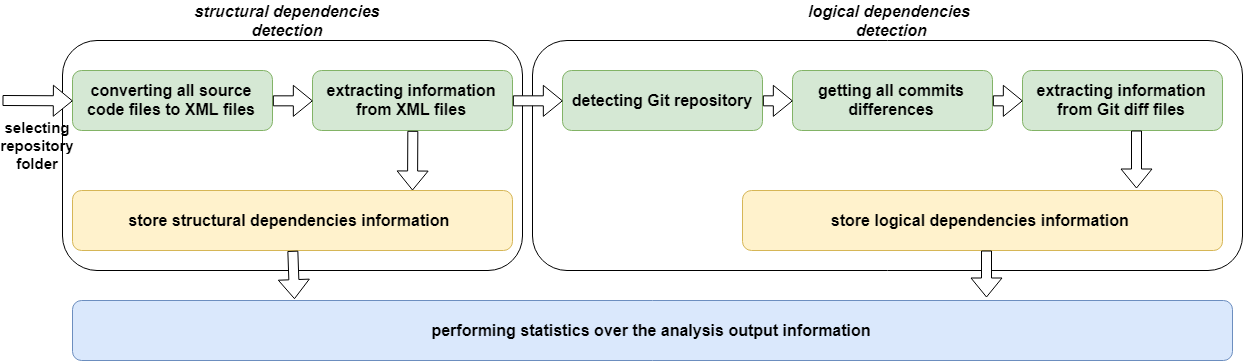
\includegraphics[width=\textwidth]{fig3.png}
\caption{Processing phases}
\label{fig:fig3}
\end{figure*}

\subsection{ Extracting structural dependencies}

Even though in some of the cases if class A depends on class B, changes in class B can produce changes in class A, but not the other way around \cite{Yu2007} . There are some cases in which if class A depends on class B,  changes in class B can produce changes in class A and viceversa. So we will consider structural dependencies as bidirectional relationships, "class A depends on class B" and "class B depends on class A". The choice of building bidirectional relationships is also motivated by the fact that we cannot establish for the moment the direction of the logical dependencies of the system. So in order to have a omogenity between the logical and structural dependencies analysis results, we will take both of the relationships types as bidirectional.
In this step the entire source code folder is scanned and only source code files are extracted in order to convert them into XML files through calls to an external tool called srcML \cite{2003:XLC:851042.857028},
\cite{Collard:2011:LTF:2067850.2068011}. All the information about classes, methods, calls to other classes are afterwards extracted from the XML files.

\subsection{Extracting logical dependencies}

The versioning system contains the long-term change history of every file. Each project change made by an individual at certain point of time is contained into a commit \cite{svn}. All the commits are stored in the versioning system cronologicaly and each commit has a parent. The parent commit is the baseline from which development began, the only exeption to this rule is the first commit which has no parent. We will take into consideration only \textit{commits that have a parent} since the first commit can include source code files that are already in development (migration from one versioning system to another) and this can introduce redundant logical links \cite{DBLP:journals/jss/AjienkaC17}. The tool looks through the main branch of the project and gets all the existing commits, for each commit a diff against the parent will be made and stored.\\ Finally after all the differences files are stored , all the files are parsed and logical dependencies are build. In addition , the number of files changed in a commit can influence the logical dependencies. A relatively big number of files changed can indicate a merge of all changes from another branch as a single commit. This can lead to a number of logical dependencies that are redundant since the files are not actually changing in the same time.The logical dependencies are splitted into three categories :\\
\textit{\textbf{Category 1:} Dependencies found in commits with less than 5 source code files changed.}\\
\textit{\textbf{Category 2:} Dependencies found in commits with more than 5 files changed but less than 20. }\\
\textit{\textbf{Category 3:} Dependencies found in commits with more than 20 files.}

Also for each category two dependencies analysis will be made:
\textit{\textbf{A:} Considering comments  as valid changes.}
\textit{\textbf{B:} Considering comments  as redundant changes. }
In the second case if class A and class B change together but the only change found is a comment change then between class A and B will not be set logical dependency.


\section{Experimental results}
\label{sec:experiments}


In this study, we have made a set of statistical analysis on a set of open-source projects in order to extract the structural and logical dependencies between classes. Table \ref{table:1} illustrates all the systems studied. The 1st column shows the projects IDs; 2nd column shows the project name; 3rd column shows the number of classes extracted; 4th column shows the number of most recent commits analysed from the active branch of each project and the 5th shows the language in which the project was developed.

\begin{table}[h]
  \centering
  \begin{tabular}{@{}ccccc@{}}
    \toprule
    ID  & Project    & Nr. of classes & Nr. of commits& Type\\
    \midrule
 \ch{1}	&	urSQL	&	39	&	89	&	java	\\
 \ch{2}	&	prettyfaces	&	257	&	207	&	java	\\
 \ch{3}	&	jbal	&	102	&	113	&	java	\\
\ch{4}	&	guavatools	&	209	&	85	&	java	\\
\ch{5}	&	monome-pages	&	196	&	280	&	java	\\
\ch{6}	&	kryo	&	289	&	743	&	java	\\
\ch{7}	&	slema	&	267	&	368	&	java	\\
\ch{8}	&	bluecove	&	386	&	1679	&	java	\\
\ch{9}	&	aima-java	&	818	&	1181	&	java	\\
\ch{10}	&	powermock	&	803	&	1512	&	java	\\
\ch{11}	&	restfb	&	713	&	1545	&	java	\\
\ch{12}	&	rxjava	&	2251	&	2468	&	java	\\
\ch{13}	&	metro-jax-ws	&	365	&	2222	&	java	\\
\ch{14}	&	mockito	&	1121	&	1572	&	java	\\
\ch{15}	&	grizzly	&	1170	&	3122	&	java	\\
\ch{16}	&	shipkit	&	222	&	1483	&	java	\\
\ch{17}	&	Tensorflow	&	1104	&	2386	&	cpp	\\

    \bottomrule
  \end{tabular}
  \caption{Summary of open source projects studied.}
   \label{table:1}
\end{table}

Table \ref{table:2}, illustrates results for commits with less than 5 files changed. The 1st column shows the projects IDs; 2nd column shows the number of structural dependencies; 3rd column shows the number logical dependencies found with comments taken into consideration as change; 4th column shows the number of logical dependencies found in col. 3 that are also structural dependencies; 5th column shows logical dependencies found without taking into consideration comments as change; finally the 6th column shows the number of logical dependencies found in col.5 that are also structural dependencies.

\begin{table}
  \centering
  \begin{tabular}{@{}cccccc@{}}
    \toprule
    ID  & SD & LD+comments & Overlaps & LD-comments & Overlaps    \\
    \midrule
 \ch{1}	&	52	&	59	&	15	&	49	&	12	\\
 \ch{2}	&	264	&	21	&	5	&	19	&	5	\\
 \ch{3}	&	106	&	27	&	2	&	27	&	2	\\
\ch{4}	&	138	&	89	&	19	&	84	&	19	\\
\ch{5}	&	250	&	239	&	40	&	217	&	38	\\
\ch{6}	&	566	&	1576	&	129	&	1488	&	126	\\
\ch{7}	&	358	&	223	&	37	&	200	&	34	\\
\ch{8}	&	447	&	687	&	61	&	619	&	58	\\
\ch{9}	&	1463	&	1063	&	101	&	963	&	86	\\
\ch{10}	&	466	&	1052	&	73	&	932	&	68	\\
\ch{11}	&	832	&	1529	&	297	&	1373	&	286	\\
\ch{12}	&	2557	&	1172	&	32	&	1107	&	31	\\
\ch{13}	&	154	&	488	&	10	&	417	&	10	\\
\ch{14}	&	541	&	2360	&	132	&	2246	&	131	\\
\ch{15}	&	2698	&	2620	&	335	&	2341	&	312	\\
\ch{16}	&	138	&	1519	&	64	&	1406	&	61	\\
\ch{17}	&	293	&	1569	&	46	&	1539	&	45	\\
    \bottomrule
  \end{tabular}
  \caption{Results for commits with less than 5 files changed}
   \label{table:2}
\end{table}


\begin{table}
  \centering
  \begin{tabular}{@{}cccccc@{}}
    \toprule
    ID  & SD & Trh 5 &Trh 10 & Trh 20    & No limit \\
    \midrule
 \ch{1}	&	52	&	59	&	145	&	288	&	415	\\
 \ch{2}	&	264	&	21	&	21	&	76	&	76	\\
 \ch{3}	&	106	&	27	&	57	&	231	&	5570	\\
\ch{4}	&	138	&	89	&	210	&	598	&	1023	\\
\ch{5}	&	250	&	239	&	824	&	1593	&	4635	\\
\ch{6}	&	566	&	1576	&	2548	&	4217	&	22437	\\
\ch{7}	&	358	&	223	&	1051	&	1756	&	6845	\\
\ch{8}	&	447	&	687	&	1421	&	2308	&	32612	\\
\ch{9}	&	1463	&	1063	&	2640	&	6257	&	156710	\\
\ch{10}	&	466	&	1052	&	2693	&	5696	&	42726	\\
\ch{11}	&	832	&	1529	&	2604	&	4184	&	32133	\\
\ch{12}	&	2557	&	1172	&	3575	&	9319	&	577118	\\
\ch{13}	&	154	&	488	&	940	&	1811	&	55837	\\
\ch{14}	&	541	&	2360	&	5871	&	9689	&	182276	\\
\ch{15}	&	2698	&	2620	&	6773	&	16058	&	218476	\\
\ch{16}	&	138	&	1519	&	3584	&	6233	&	22145	\\
\ch{17}	&	293	&	1569	&	3253	&	5667	&	32347	\\
\midrule
Overlapping Avg \\ LD with SD	&	&	13,76	&	23,26	&	36,04	&	66,48	\\
    \bottomrule
  \end{tabular}
  \caption{Logical dependencies for different types of thresholds, case with comments}
   \label{table:5}
\end{table}



\begin{table}
  \centering
  \begin{tabular}{@{}cccccc@{}}
    \toprule
       ID  & SD & Trh 5 &Trh 10 & Trh 20    & No limit \\
    \midrule
 \ch{1}	&	52	&	49	&	121	&	257	&	319	\\
 \ch{2}	&	264	&	19	&	19	&	74	&	74	\\
 \ch{3}	&	106	&	27	&	33	&	171	&	5553	\\
\ch{4}	&	138	&	84	&	194	&	566	&	991	\\
\ch{5}	&	250	&	217	&	712	&	1327	&	4004	\\
\ch{6}	&	566	&	1488	&	2307	&	3928	&	20396	\\
\ch{7}	&	358	&	200	&	918	&	1502	&	4751	\\
\ch{8}	&	447	&	619	&	1255	&	2066	&	31879	\\
\ch{9}	&	1463	&	963	&	2374	&	5632	&	149531	\\
\ch{10}	&	466	&	932	&	2399	&	4729	&	35846	\\
\ch{11}	&	832	&	1373	&	2305	&	3618	&	28401	\\
\ch{12}	&	2557	&	1107	&	3340	&	7948	&	333585	\\
\ch{13}	&	154	&	417	&	758	&	1407	&	51894	\\
\ch{14}	&	541	&	2246	&	5424	&	8504	&	148053	\\
\ch{15}	&	2698	&	2341	&	5716	&	12486	&	178262	\\
\ch{16}	&	138	&	1406	&	3161	&	5475	&	20215	\\
\ch{17}	&	293	&	1539	&	3195	&	5578	&	29720	\\
\midrule
Overlapping Avg \\ LD with SD	&	&	13,76	&	22,14	&	34,38	&	63,95	\\
    \bottomrule
  \end{tabular}
  \caption{Logical dependencies for different types of thresholds, case without comments}
   \label{table:6}
\end{table}



\begin{table}
  \centering
  \begin{tabular}{@{}cccc@{}}
    \toprule
    ID  & 1 link &2 links & 3 links  \\
    \midrule
 \ch{1}	&	28,85	&	15,38	&	1,92		\\
 \ch{2}	&	1,89	&	0,76	&	0,38		\\
 \ch{3}	&	1,89	&	0,94	&	0,00		\\
\ch{4}	&	13,77	&	2,17	&	1,45		\\
\ch{5}	&	16,00	&	8,00	&	3,20		\\
\ch{6}	&	22,79	&	12,54	&	4,24		\\
\ch{7}	&	10,34	&	3,63	&	0,56		\\
\ch{8}	&	13,65	&	5,82	&	2,68		\\
\ch{9}	&	6,90	&	1,78	&	0,27		\\
\ch{10}	&	15,67	&	2,58	&	1,07		\\
\ch{11}	&	35,70	&	26,56	&	9,38		\\
\ch{12}	&	1,25	&	0,82	&	0,35		\\
\ch{13}	&	6,49	&	2,60	&	1,30		\\
\ch{14}	&	24,40	&	14,05	&	6,28		\\
\ch{15}	&	12,42	&	4,11	&	2,04		\\
\ch{16}	&	46,38	&	29,71	&	14,49		\\
\ch{17}	&	15,70	&	9,56	&	5,46		\\
\midrule
Avg	&	13,76	&	4,11	&	1,92	\\	
    \bottomrule
  \end{tabular}
  \caption{Overlapping results in percentage for logical dependencies extracted from commits with less than 5 files changed, splitted by numbers of occurrences }
   \label{table:10}
\end{table}



\begin{table}
  \centering
  \begin{tabular}{@{}cccc@{}}
    \toprule
    ID  & 1 link &2 links & 3 links  \\
    \midrule
 \ch{1}	&	76,92	&	46,15	&	21,15		\\
 \ch{2}	&	1,89	&	0,76	&	0,38		\\
 \ch{3}	&	85,85	&	84,91	&	83,96		\\
\ch{4}	&	70,29	&	15,22	&	10,87		\\
\ch{5}	&	69,60	&	58,40	&	44,80		\\
\ch{6}	&	65,55	&	42,05	&	30,57		\\
\ch{7}	&	66,48	&	32,68	&	18,99		\\
\ch{8}	&	64,88	&	43,40	&	20,58		\\
\ch{9}	&	75,32	&	58,58	&	41,90		\\
\ch{10}	&	57,73	&	30,69	&	19,53		\\
\ch{11}	&	81,49	&	64,66	&	37,98		\\
\ch{12}	&	14,74	&	8,80	&	5,91		\\
\ch{13}	&	33,12	&	9,74	&	7,79		\\
\ch{14}	&	67,28	&	45,84	&	26,80		\\
\ch{15}	&	52,85	&	33,80	&	22,65		\\
\ch{16}	&	80,43	&	71,01	&	55,07		\\
\ch{17}	&	24,57	&	18,43	&	17,06		\\
\midrule
Avg	&	66,48	&	42,04	&	21,15 \\		
    \bottomrule
  \end{tabular}
  \caption{Overlapping results in percentage for logical dependencies extracted from all commits, splitted by numbers of occurrences }
   \label{table:11}
\end{table}


\section{Discussion}
\label{sec:discussion}


This section presents the results of the three analyses, performed on the selected projects (\ref{table:1}). The purpose is to answer the three research questions outlined in section \ref{sec:question}.

\textit{\textbf{Question 1}}. How the number of source files changed in a commit can influence the logical dependencies of the system and the overlapping rates with the structural dependencies.

Based on the results presented in tables \ref{table:5} and \ref{table:6}, from section \ref{sec:experiments}, the number of changed files taken into consideration has an important influence over the overall rates of the logical and structural dependencies overlaps. If no threshold is set for the number of files then we can affirm that a significant number of structural dependencies are also logical. In table \ref{table:5} we have obtained an overlap of structural and logical dependencies of 63,95\% which is with 41,81\% more than if consider only commits with less then 5 source code files changed per commit (Figure \ref{fig:figvenn}) and with 22,14\% more if consider only commits with more then 5 and less then 20 source code files changed per commit.

\begin{figure*}[h]
\centering
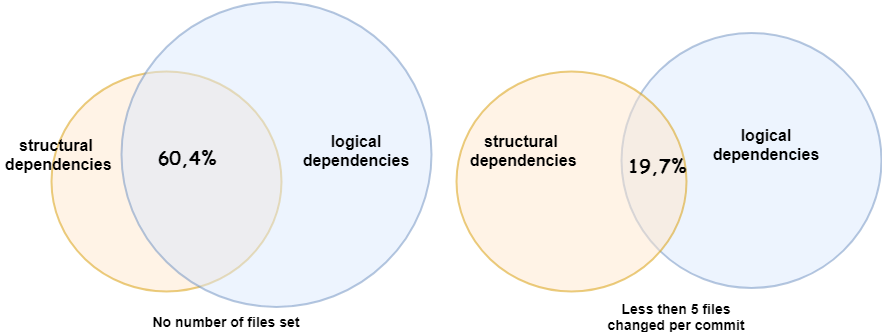
\includegraphics[scale=0.5]{fig4.png}
\caption{Venn diagrams of the overlapping rates with comments taken into consideration as change}
\label{fig:figvenn}
\end{figure*}


\textit{\textbf{Question 2}}. Considering comments can lead to additional logical dependencies ? How many logical dependencies are introduced by considering comment changes as valid changes and in what percentage this can influence the final result ?

Table \ref{table:comm} illustrates the percentages rates extracted from tables \ref{table:5} and \ref{table:6} from section \ref{sec:experiments}. As it was specified in the tables description , the percentages rates are the number of structural and logical dependencies overlaps, reported to the total number of structural dependencies. How it can be seen, the overlapping rates are also influenced by the comments filtering but in a small percentage. The rates are with aprox 2\% lower if comments are not taken into consideration as a change. (Figure \ref{fig:figvenn2})


\begin{table}
  \centering
  \begin{tabular}{@{}c||cc@{}}
    \toprule
       Category & With comments & Without comments  \\
    \midrule
less 5	&	13,76\% &	13,76	\%	\\
more 5 less 20	&	23,26\% &	22,14\%\\
more 20	&	36,04\%	&	34,38\%\\
total & 66,48\% &63,95\% \\
    \bottomrule
  \end{tabular}
  \caption{Average percentages rates with and without considering comments as valid changes.}
   \label{table:comm}
\end{table}

\begin{figure*}[htb]
\centering
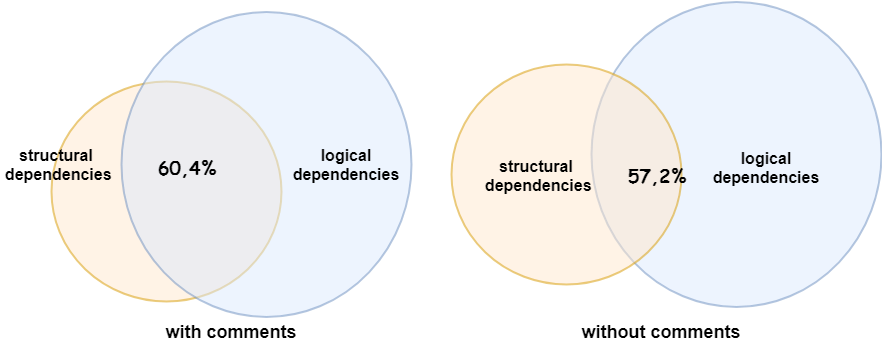
\includegraphics[scale=0.5]{figvenn2.png}
\caption{Venn diagrams of the overlapping rates with comments and without comments taken into consideration.}
\label{fig:figvenn2}
\end{figure*}



\textit{\textbf{Question 3}}. One occurrence of a logical dependency is enough to consider it as valid ? If we consider only logical dependencies with more then one occurrence as valid, the results are influenced in a significant way ?

Table \ref{table:10} and \ref{table:11} from chapter Experimental Results,  illustrates results in percentages, reported to the structural dependencies, of the analysis for all the systems when logical dependencies where build with/ without comments taken into consideration as change and multiple occurrences of logical dependencies taken into consideration as valid dependencies. Based on the experimental results averages \ref{table:14} , we can affirm that the results are with approx 50\% lower after filtering \ref{table:comm}. This indicates that a lot of logical dependencies are the result of a single commit in which the two elements of the dependency where changed together. 

If we look at the average rates of projects 13, 15, 16, 18 we can observe that the difference is much smaller (15-20\%), the only thing that those projects have in common is the size and the number of commits compared to the other ones from the list, the size and the number of commits of the projects mentioned above are relatively big. 

This can lead to the conclusion that, if the project studied has a relatively small amount of commits ( Project ID 8.), the probability to find multiple updates of the same classes in the same time can be small, so filtering after the number of occurrences can lead to filtering all the logical dependencies extracted. (Figure \ref{fig:figvenn3})

\begin{table}
  \centering
  \begin{tabular}{@{}c||cc@{}}
    \toprule
       Category & With comments & Without comments  \\
    \midrule
less 5	&	9,09\% &	8,67\%	\\
more 5 less 20	&	15,87\% &	13,29\%\\
more 20	&	18,8\%	&	16,52\%\\
total &39,1\% & 35,38\% \\
    \bottomrule
  \end{tabular}
  \caption{Overall percentages rates by filtering the logical dependencies occurrences. }
   \label{table:14}
\end{table}


\begin{figure*}[htb]
\centering
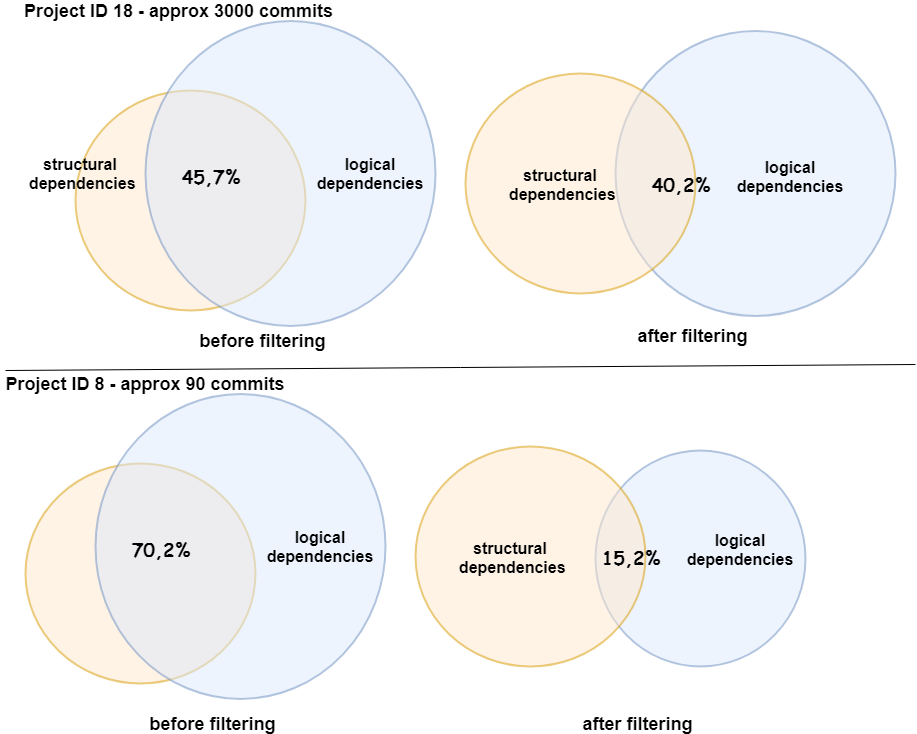
\includegraphics[scale=0.5]{figvenn3.png}
\caption{Impact of logical dependencies occurrences filtering on projects with different sizes.}
\label{fig:figvenn3}
\end{figure*}


As a conclusion, it results that large number of structural dependencies are doubled by logical or not, this number is particularly influenced by the number of files that participate in a commit that taken into consideration. It also results that taken or not comments as change, the final results are not influenced in a big percentage.  

In this research work we have tried to identify methods to acquire the most relevant logical dependencies from the system so that can be used in the future for architectural reconstruction, that is currently based only on the information provided by structural dependencies.

For future work, we will investigate the cause for the large number of logical dependencies which are not overlapping with structural dependencies. As we can see in tables \ref{table:ldol1} and \ref{table:ldol2}, where the percentages are reported to the logical dependencies, only a small amount (aprox 10\%) of logical dependencies are also structural .

 In this work we have extracted structural dependencies from the last revision of the system but logical dependencies from all the revisions of the system. We will study also structural dependencies from all the revisions of the system since some logical dependencies may have been also structural on previos revisions of the system but not in the current one. If we take into consideration also structural dependencies from previous revisions then the overlapping rate between logical and structural dependencies will probably increase.



\section {Threats to validity}
\label{sec:validity}


bla threats

\section{Conclusion}
\label{sec:Conclusion}
   
	
bla final concl


% conference papers do not normally have an appendix


% use section* for acknowledgment
%\section*{Acknowledgment}
%
%This work was partially supported by a grant of the Romanian National Authority for Scientific Research and Innovation, CNCS/CCCDI UEFISCDI, project number PN-III-P2-2.1-PED-2016-0999, within PNCDI III.


% trigger a \newpage just before the given reference
% number - used to balance the columns on the last page
% adjust value as needed - may need to be readjusted if
% the document is modified later
%\IEEEtriggeratref{8}
% The "triggered" command can be changed if desired:
%\IEEEtriggercmd{\enlargethispage{-5in}}

% references section

% can use a bibliography generated by BibTeX as a .bbl file
% BibTeX documentation can be easily obtained at:
% http://mirror.ctan.org/biblio/bibtex/contrib/doc/
% The IEEEtran BibTeX style support page is at:
% http://www.michaelshell.org/tex/ieeetran/bibtex/
\bibliographystyle{IEEEtran}
% argument is your BibTeX string definitions and bibliography database(s)
\bibliography{IEEEabrv,logicaldepd}
%
% <OR> manually copy in the resultant .bbl file
% set second argument of \begin to the number of references
% (used to reserve space for the reference number labels box)
%\begin{thebibliography}{1}
%
%\bibitem{IEEEhowto:kopka}
%H.~Kopka and P.~W. Daly, \emph{A Guide to \LaTeX}, 3rd~ed.\hskip 1em plus
% 0.5em minus 0.4em\relax Harlow, England: Addison-Wesley, 1999.
%
%\end{thebibliography}




% that's all folks
\end{document}


